
%TODO Skriv litt om: halv dag.
%
% PLAN:
% - ta med "propagating of kappa". At metoden brukt er antagelig ikkje den mest effektive, men det gjøres likt for å lage det meir egna for sammenligning.(ligger i implementation.tex)
% - ta med "om oppsamling av kappa" (ligger i implementation.tex)

% Kan sei at dette er "original work by the author." Dette kan ivertfall brukes når dette kapittel blir referert til!

%TODO Skriv om mealy automata, ANN, input som aktivitetsvariabel for 1.gen. og 2.gen. ANN og state som aktivitetsvariabel for 3.gen. ANN.
% 	Kan da skrive at denne modellen har aktivitetsvariabel for både state og input (Kappa, dDepolAtStartOfTimeWindow), og kan dermed lett transformerer KANN's aktivitetsvariabel over til 1g.ANN, 2g.ANN og 3g.ANN!
% 	Sjå [ ref_asdf2143@ANN ] i ANN.tex.

%*********************** KANN ***************************
\section{KANN design and implementation}
\label{secKANN}
	
	%KANSKJE NESTE subsection er INNLEDNING til section? ELLER kanskej eg heller skal skrive motivatorisk? (SKrive om mine håp for modellen..)
	INNLEDNING: Mens SANN kjører en direkte simulering av mekanismene i neuronet, har eg i dette prosjektet modellert mekanismene.
	Ved hjelp av matematikken fra sec. [ref->modellering-kap] er ideen at det er mulig å lage eit meir effektivt, eller på andre måter bedre, ANN.
% 		Skriv at eg vil gjøre eit forsøk på å lage eit ANN med flyttalsvariabel som propagerer (og kvifor), men med state for å gi spike timing.
% 		%	x Forrige kapittel: Skriv om grunnen til å gå vidare til ANN med informasjon om relativ spike timing ALLEREDE ER gått gjennom. REFERER. Nevn STDP, LFPO.

	Skriv først innledning, med mål om å sette meg og leser på samme utgangsnivå.
	Skrive litt om kvifor eg tenker det er lurt å gå videre fra SANN.
	Modellere det, og bruke formalisert matematikk fremfor å ha ei naiv direkte simulering av mekanismene i enkeltneuronet.
	%Skrive at eg desverre ikkje fekk tid til syn.P. i dette prosjektet?

	Skriv også det som står i TODO over, eller i ANN.tex: [ ref\_asdf2143@ANN ]% Søk etter ref_asdf2143@ANN i fila ANN.tex.
	"As we will see, this new model for ANN have both a state and output given by the last time iteration's state and the input to the node. 
	This gives that the node is able to communicate with all the previous forms of ANN, and might serve as an important transform between different models of ANN."
	%XXX Dette er vel heller analyse, forresten. TODO Skriv det over i analyse/comparison kapittel.
	% MEN kanskje også her?

 		\subsection{The Activity Variable} %TODO I Implementasjon:SANN er det viktig at eg skriver at aktivitetsvariabelen er brukt til depol til noden. (da blir teksten under rett)
	When the neuron is modelled as a LIF neuron, the depolarization of the node will behave much like a condencator. 
	The depolarization value of a biological neuron will go towards some value $\kappa$ for a constant, continous input.
	% This value is given by the input and the grade of leakiness.
	% Ta vekk den over(kommentert ut), eller siste bit av den under.

	As seen in section \ref{secMatematiskModelleringAvBioNeuron}, $\kappa$ is given by the input and the grade of leakiness of a node.
	For changing $\kappa$, we introduced the concept of \emph{time window}. 
	A time window is defined as a period of time where $\kappa$ is constant within the current interspike period (see section \ref{ssecVariableInputBetweenSpikes}).
	By using eq. \eqref{eqVerdiligninga} it is possible to find the depolarization value of the node at any time $t \, \epsilon \, p_{isi}$.
	We can therefore use $\kappa$ as the node's activity variable.

	%TODO TODO Skriv på nytt! Skriv også at det er mulig å kalkulere f=p^{-1}. Desse tre elementa gjør det mulig å kommunisere med alle de tre tiligere generasjonene ANN (men ikkje skriv "tidligere")
	If $\kappa$ is used as the activity variable, more than the depolarization value of the node can be calculated by its activity variable. 
	In section \ref{secMatematiskModelleringAvBioNeuron} we have seen that both the firing time and the period corresponding to the activity variable can be calculated when we use $\kappa$ as the activity variable.
	%By using that the frequency is the inverse of the period,  it ...
	It is therefore possible to use a node based on the mathematics present in section \ref{secMatematiskModelleringAvBioNeuron} as an interface to each of the other generations ANN.
	% In section \ref{secMatematiskModelleringAvBioNeuron} we have seen that from kappa, both the value of the node (the ``depolartization'') and the estimated firing time can be calculated.

	To interface with a second generation ANN, we can use that the frequency is the inverse of the period. The period is calculated from eq. \eqref{eqHeilePerioden}.
	The $\kappa$N can as easily be used to get input from as sending output to a node of a second generation ANN. %TODO TODO Dette stemmer ikkje! xxx

	% TA VEKK: Interfacing with a node of the first XXX Dersom eg ikkje HEILT forstår 1.gen. noder.
	For interfacing with a node of the first or third generation ANN, the spike time of the node will be used. % ref_123@i_KANN TODO enten forstå 1.gen HEILT, eller ta bort dette. (her og over("..all other gen. ANN"))
	As the node ``fires an acion potential'', and sends output thourgh all its output synapses at the time calculated by eq. \eqref{eqRemainderOfPeriod}, the node could work as an interface to a node of a third generation ANN. 
	Here special synapses needs to be devised for the transmission to SANN nodes. 
	The connections between the $\kappa$N and the SN will use the transmission sceme from SANN, where the synapse transmit its synaptic weight to the postsynaptic node. 
	Transmissons from the SN to  the $\kappa$N is a little more complex. Here the equivalent $\kappa$ resulting in the level of transmission needs to be calculated, and from this the level of transmission.
	Development of a transductor node between different generations of ANN will not be procecuted further, as this falls outside the scope of this project.

	% TA VEKK? Blir så veldig svevende.. Fin tekst, men får følelsen av at dette er fiction.
	%The first generation ANN were stateless, and the ouput only varied with the immediate input. 
	%This demands a different kind of transduction mechanism, but because the first generation ANN could be said to be obsolete, no more time will be used on this.
	%The most important 
	%
	%In a $\kappa$N, the activity variable can therefore represent $\kappa$ instead of the depolarization of a corrsponding neuron.
	
	If a suitable scheduler is devised $\kappa$ could be used effectively for planning, or ``estimating'' the firing time of the node.
	The rationale behind the use of the word estimate is that the estimated firing time will change every time the activity variable changes, possibly before the initially calculated firing time. 
	The firing time is then updated. 
	The first firing times computed by eq. \eqref{eqRemainderOfPeriod} is therefore but a naive estimate of the firing time of the node.
	As the time of firing of the node approaches, the estimated firing time becomes more certain.
	When the present time iteration is the same as the estimated firing time, the estimated firing time is exact; The node's value is now above firing threshold.
	
	%The estimated firing time is computed by eq. \eqref{eqRemainderOfPeriod}, and will be firing time of the node given that the present time window last until firing (no change in $\kappa$ for the remainder of the period).

	%Because of time limitations for this project, effectivity analysis have not been conducted. %Litt rart språk! XXX conduct conduct!

	
	%\subsection{Updating $\kappa$} %Calculation and recalculation of $\kappa$
	\subsection{Synaptic transmission}
		%TODO Skriv om, med kontinuerlig tanke på kappaANN. F.eks. : in biology, AND IN SANN, a synaptic ...

		% skrive om korleis synaptic transmission fåregår (generellt (om at $\kappa_{ij} = \frac{W_{ij}}{p_{pre}}$ ).
		In biology and in the SANN model, a synaptic transmission change the value of the postsynaptic node.
		Because we do not use the depolarization value as the activity variable in a $\kappa$N, this form of synaptic transmission makes the model a bleak copy of SANN.   %XXX eller bare " a compy of SANN." Nee. Men bleak er dårlig.
																							% , this form of synaptic transmission will not work. %TODO TODO SKriv om! XXX
		A better approach is to develop a separate model for synaptic transmisson in $\kappa$ANN.

		For second generation ANNs, synaptic transmission is defined as the synaptic weight times the number of incoming spikes per time step.
		This can be formalized as
		\begin{equation}
			u_{ij}(t) \, = f_{j} \cdot w_{ij} \cdot \Delta t
			\label{eqSynapticTransmissionFor2genANN}
		\end{equation}
		Where $u_{ij}(t)$ is the control signal from node $j$ to node $i$, $w_{ij}$ is the size of the synaptic weight %between node $j$ and node $i$ 
			and $f_j$ is the presynaptic node's firing frequency.
		Because $\kappa$ANN contains elements from both the second and third generation ANN, % eller :  {ANN and from SANN} %Litt dristig å sammenligne meg med 3.gen som en anna modell? (men det er jo sant..)
																							 we can not ute either of these transmisson rules.

		%Eq. \eqref{eqSynapticTransmissionFor2genANN} states that the contribution from node $j$ to node $i$'s activity variable is a function of the frequency of the presynaptic neuron.
		Inspired by \eqref{eqSynapticTransmissionFor2genANN}, we define synaptic transmisson in $\kappa$ANN as the synaptic weight times the activity variable's corresponding frequency.
		By combining eq. \eqref{eqHeilePerioden} and \eqref{eqSynapticTransmissionFor2genANN} and using that $f_j = \frac{1}{p(\kappa_j)}$ we get
		\begin{equation}
			\kappa_{ij}(\Delta t) = \frac{ w_{ij} }{ p_{isi}(\kappa_j)} \cdot \Delta t  %XXX  Verifiser at alt passer inn, no (at var.navn er rett osv)
		\end{equation}
 		
		$\kappa_{ij}$ here defines the synaptic transmission in the connection between node $j$ and node $i$.
		% XXX Bare ta med når du finner ut HEILT kva som er effekta av det motastte XXX :  If the time step large enough, we can define that each synaptic transmission lasts for one time step.
		For simulations with constant time steps, $\Delta t$ is constant and can be incoorporated into the synaptic weight $w_{ij}$.
		We get the equation used for synaptic transmission in $\kappa$ANN.
		%If we define the transmission of the synapse between node $j$ and node $i$ as $\kappa_{ij}$ we get the equation for synaptic transmission:
		\begin{equation}
			\kappa_{ij} = \frac{ w_{ij} }{ p(\kappa_j)}
			\label{eqSynapticTransmissionForKANN}
		\end{equation}

		This equation is a simplification of the biological synapse, as it does not take into account the timing of successive transmissons and other time elements of transmisson 
																							%short--term synaptic plasticity as a consequence of rapid transmissions (see appendix \ref{appendixSecPresynapticSynapticPartOfTransmission}).
			(see appendix \ref{appendixSecPresynapticSynapticPartOfTransmission} for an introduction to synaptic potentiation). 
																					%a discussion of time elements in transmission in the biological synapse ).%eller heile appendix A (syn. trans.)

		%TODO TODO TODO TODO ENTEN : skriv først at for ei synapse-neuron så er K_i lik K_ij
		%TODO TODO TODO TODO ELLER : Skriv direkte at K_i er summen av input (bruk ord som lineær karrakteristikk, superposisjon, osv.)
		The typical neuron has numerous input synapses. 
		%How does \eqref{eqSynapticTransmissionForKANN} expand to multiple synapses?
		%
		%TODO Skriv om: No er det for sein, og eg tenker ikkje beint.
		As for temporally separated input, the synapses' total effect of multiple transmissions is modelled as a linear carracteristic. %TODO TODO Skriv kvifor / begrunn dette valget!
		%This gives that the postsynaptic potential is the sum over all the input nodes' transmission.
		% %Just as the input of many ``simultaneous'' transmissions has a linear carracteristic, the input through multiple synapses be 
		%
		%This model of synaptic transmission does not take into account 
		For nodes with multiple input edges, the activity variable $\kappa_i$ is the sum of the contribution from each of its input synapses.
		%jeje Skriv om det på slutten, setninga over. Kanskje  					 is the sum of all the contributions from different input synapses. (?) XXX XXX
		\begin{equation}
			\kappa_i = \sum_j{\kappa_{ij}}
			\label{eqSumOfKij}
		\end{equation}

		The effect of each synaptic transmission can therefore be decoupled from the other synaptic transmissions when calculating the postsynaptic effect of a transmisson.
																				%the rest in the calculation of the postsynaptic node's activity variable, $\kappa_i$.



		%In discrete--time systems, we can define every synaptic transmission to last for one time iteration (if the time step is large enough).  % MED ELLER IKKJE: "(if the time step is large enough)" ??? XXX
		%This causes $\Delta t$ to become constant. We can incoorporate this constant into $W_{ij}$.

%		For an ANN based on the activity variable $\kappa$, as previously introduced in chapter \ref{secMatematiskModelleringAvBioNeuron} %TODO Sjekk denne  referansen bedre / skriv bedre (?).
%		eq. \eqref{eq SynapticTransmission} is highly relevant.  % highly relevant skurrer litt. Det er veldig relevant. Finn synonym..
%		If we define $\Delta t$ to be some constant, and incoorporate this constant into $W_{ij}$, we get the equation for the synaptic transmission of the activity variable.
%		We call the size of this transmission for $\kappa_{ij}$.


		%For nodes with multiple input synapses, the activity variable $\kappa$ is the sum of all the contributions from different synapses. %VERIFISER DETTE! Vær heilt heilt sikker på at K=sum(K_ij)
		%We can write this mathematically as 
		%\begin{equation}
		%	\label{eqSumOfKij}
		%	\kappa_i = \sum_j{\kappa_{ij}}
		%\end{equation}
		%
		%In this way the synaptic transmission of the individual synapses can be decoupled from the postsynaptic activity variable, $\kappa_i$.
		

		\subsection{The Postsynaptic Effect of Synaptic Transmissons}
			\label{ssecSynInputToANodeKANN}
			Equation \eqref{eqSumOfKij} defines the postsynaptic effect of transmissions from multiple input synapses.
			In pragmatic ANNs the effectivity of the implementation is an issue, and an attempt has been made to make the calculation of the node's activity variable more effective.
			
			% As we will see, ... (det under) .  		No fremstår det som en ubegrunna påstand. XXX
			If we define a transmission in the edge as the derived of the corresponding synaptic transmission, we will see that this makes the implementation more effective.
																												%updating the postsynaptic node's activity variable after a transmission becomes more effective.
			The synaptic transmission now becomes the integral of all the edge's transmissions, modelled by %eq. \eqref{eqSynapticTransmissionAsSumOfEdgeTransmissions}.      %, and is defined as
			\begin{equation}
				\kappa_{ij} = \sum_t{u_{ij}(\kappa_j)}
				%\kappa_{ij} = \int{u_{ij}(\kappa_j)} \, \mathrm{d}t
				\label{eqSynapticTransmissionAsSumOfEdgeTransmissions}
			\end{equation}
			
			Where $u_{ij}(\kappa_j)$ is the transmission through the edge.
			This involves that a new transission updates $\kappa_{ij}$ by adding its value to the current $\kappa_{ij}$.
			%As the postsynaptic node's activity variable is the sum of all the synaptic transmissions, as defined in \eqref{eqSumOfKij}, transmission through 
			As the postsynaptic node's activity variable is the sum of all the synaptic transmissions, and each synaptic transmission is the integral of all the transmissions through the edge, 
				$\kappa_i$ can be updated by simply adding the new edge transmission to $\kappa_i$.
			%VIKTIG XXX Skriv litt om at Kappa er fullstendig time-invariant. Viktig for modellen, og ikkje heilt selvsagt!

			In the previous paragraph, we used two 		 different expressions for transmission through a connection between two nodes. 
			%We have in the previous paragraph used two
			The synaptic transmission $\kappa_{ij}$ is used as the amount $\kappa_j$ transmitted by the connection between node $j$ and node $i$. 
			The edge transmission $u_{ij}(\kappa_j)$ is used as the transmission from node $j$ to node $u$ in the implementation. 
			These two transmissions differ if the implementation's solution is different than a direct implementation of eq. \eqref{eqSynapticTransmissionAsSumOfEdgeTransmissions}.
			%A discussion 
			% FEIL: The choice for this implementation is presented in the next section (sec. \ref{ssecImpOfSynTransmissionKANNN}).
			For this implementation the edge transmission is previously defined as the change in synaptic transmission. 
			%The fact that these transmissions differ follows a solution for making the implementation more effetive.


			Each edge's transmission is completely decoupled from the others' transmissions.
			Each synapse's transmissions can therefore be calcutated separately.
			In an object mode, this is very good for encapsulation as each synapse can update its own $\kappa_{ij}$.
			%This is completely decoupled from the other transmissions, and each edge transmission can be calculated by the edge at the time of transmission. 
			%This is wery good for encapsulation in an object oriented programming language.

			After each time iteration, the postsynaptic node's activity variable is updated as the sum of all the synapses with an altered level of transmission.
																																%  changed         ?

			%For synapses transmitting the derived of $\kappa_{ij}$ we only have to integrate this change of transmission from all the input synapses with a changed level of transmission, and get
			\begin{equation}
				\kappa_i = \sum_c{\kappa_{ic}}
				\label{eqSynapticTransmissionForKANNimplementation}
			\end{equation}
			Where $\{c\}$ is a subset of $\{j\}$ consisting of all the presynaptic neurons where the activity variable has been updated.

			% KANSKJE: skrive at kappa er tidsinvariant, og varierer bare med kappa_ij. Dette gjør ting lettere.

			%In the implementation of $\kappa$ANN we call the nodes for K\_auron.
			%The synaptic input for the activity variable of a K\_auron is defined by \eqref{eqSumOfKij}.
			% %To avoid having to recalculate $\kappa_i$ from \eqref{eqSumOfKij} every time the transmission of a synapse changes, we can implement synaptic transmission as the transmission of the derived of $\kappa_{ij}$.
			%To avoid recalculation of $\kappa_i$ from all the input synapses when one synapse changes its transmission, this implementation defines edge transmission as the derived of $\kappa_{ij}$.
			%Now the postsynaptic $\kappa_i$ can be calculated without summing all the synapse inputs after changed input at one of its edges.
			% %In this case the postsynaptic $\kappa$ can be recalucated without summing all the synaptic inputs every time one synapse changes its transmission.

			To sum up the analysis in this seciton, edge transmission of the implementation is defines as  $u_{ij}(\kappa_j) = \Delta K_{ij}$.
			For each edge transmission the synaptic transmission $\kappa_{ij}$ is the integral of all edge transmissions, and is updated by simply adding the new edge transmission.
			The postsynaptic node's activity variable $\kappa_i$ is the sum of all it's input transmissions, and is updated by the same principle; %var: , and can be updated ..
				After an edge transmission $u_{ij}(\kappa_j)$, $\kappa_i$ is updated by simply adding $u_{ij}(\kappa_j)$. 
			%The operation of taking the sum over all the node's input synapses after a change in one input transmission is thus avoided.
			%The operation of taking the sum over all the node's input synapses, after a change in transmission for a subset of the input synapses is thus avoided.
			 The operation of taking the sum over all the node's input synapses after a change in one $\kappa_{ij}$ is thus avoided.

			%We can, in other words, add the change in synaptic transmission, $\Delta K_{ij}$, to the postsynaptic activity variable to get the updated activity variable, $\kappa_i$.
			%The edge transmission in the implementation is defined as $u_{ij}(\kappa_j) = \Delta K_{ij}$, so for each edge transmission the postsynaptic node's activity variable is by simply adding $u_{ij}(\kappa_j)$.
			%This can be done at the time of each transmission, and without having to consider any of the other synaptic transmissions to the node.
			
			%XX Skal eg skrive dette her: XXX Dette står vel i neste avsnitt?
			%If we wait until after the current time iteration before calculating the effects of the changed kappa, much calculations will be saved.




			\subsection{Implementation of Synaptic Transmission}
			\label{ssecImpOfSynTransmissionKANNN}
	
	%		Begynn med å skrive at det er er vankelig å vite når det skal skje. Diskuter litt fram og tilbake som intro til section. %TODO 
	
			The synaptic transmission is given by $\kappa_{ij} = w_{ij} \, \cdot \, p_{isi}^{-1}(\kappa_j)$, the synaptic weight multiplied by the inverse of the inter--spike period.
			%In this implementation, $\kappa$ is used as the activity variable instead of the node's depolarization, and an other transmission scheme needs to be devised.
			Edge transmission is in this implementation defined as the change in synaptic transmission, or $u_{ij}(\kappa_j) = \Delta \kappa_{ij}$
			%This itroduces mechanisms that makes it redundant to perform the sum over all the node's input synapses every time one synapse's $\kappa_{ij}$ is updated.
			This introduces mechanisms that makes computational of the sum over alle the node's input synapses redundant, as more effective methods are used. %TODO skriv om!
			%TODO finn ut korleis eg skal skrive det over / which of dei to setningene eg skal basere setninga på..
	
			%%\subsubsection{Implementation of transmission through a synapse} % Vettafaen om denne skal være med. Gjorde om fra å være en kommentar, no..
			When implementing synaptic transissions, equation \eqref{eqSynapticTransmissionForKANN} is considered first.
			This equation is based on the presynaptic inter--spike period and the synaptic weight of the edge, elements that are available from the presynaptic node and the synapse itself.
			At the time of transmission, the edge transmission is further calculated as the change in $\kappa_{ij}$.
			
			When $\kappa$ is changed, a new time window is commenced. 
			The node's initial depolarization in the new time window is calculated as the value of the node at the end of the previous time window.
			With the starting value for the node's depolarization, the further depolarization curve and the estimated firing time of the node can be calculated by eq. \eqref{eqVerdiligninga} and \eqref{eqRemainderOfPeriod}.

			A time step is defined as the smallest iteration in time.
			The first time the effect of a changed $\kappa$ may appear is thus after the current time iteration.
			As we potentially get multiple edge transmissions each time iteration, many calculations can be saved by calculating the effect of changed $\kappa$ after the current time iteration.
			For every edge transmission we only add the new transmission to the current $\kappa$.

			Every time a node's $\kappa$ is changed, a pointer to the node is inserted into a list \emph{pCalculateTaskQue}, introduced in section \ref{ssecCalcultaionTaskQue}.
			This list is a static element of \emph{time\_class}, and only one instance of the list is constructed. 
\begin{lstlisting}
static std::list<timeInterface*> pCalculateTaskQue;
\end{lstlisting}
			This list is specifically designed to keep an overwiev of \emph{timeInterface} derived classes in need of post--iteration calculations. %todo skriv om!
%			One example of this is a node after a changed $\kappa$. %in it's activity variable, $\kappa$.
			Before time is iterated by \emph{time\_classes::doTask()}, \emph{time\_class::doCalculation()} is called.

			The first task of \emph{time\_class::doCalculation()} is to make shure that every entry of \emph{pCalculateTaskQue} is unique, by removing every duplicate entries of each element of the list.
			After this, \emph{time\_class::doCalculation()} calls each entry's doCalculation() function.
			% TODO Neste to linjene hører heime i design.tex:
			The \emph{doCalculation()} function is defined as a pure virtual fucion in the \emph{timeInterface} class, assuring that every object of a derived class have defined it own \emph{doCalculation()} function.
			%meaning that every class inheriting this function have to implement the action of this function for the class.
			%If it does not, the derived class will inherit the interface aspect of \emph{timeInterface}, and cannot be made an instance of. %TODO Skriv om!
		
			In class \emph{K\_auron},  the \emph{doCalculation()} member function is responcible for updating variables dependent on $\kappa$.
			%The \emph{doCalculation()} member function of class \emph{K\_auron} calculates the effect of a changed $\kappa$.
			In this way equation \eqref{eqSynapticTransmissionForKANNimplementation} is implemented during each time step, and the calculation of the updated effect of the new $\kappa$ is executed at the end of the time step.
			The more strenuous task of calculating the initial values of the new time window and the effect of the changed $\kappa$ for the node is thus called at most once for every time iteration.

%\begin{lstlisting}
%static std::list<timeInterface*> pCalculateTaskQue;
%\end{lstlisting}


	
% Setninger som inneheld aspekt som eg ikkje har dekka:
		%	When $\kappa_i$ changes for a node, we need to recalculate the inverse of the period for this new $\kappa_i$ to get the synaptic transmissions right.
		% Synaptisk transmission er resultat av p^-1 Dette er ikkje skrevet over.

		% uvisst kva delay før propagation av kappa skal være.


	
	

% _____________________ fiksa til hit __________________________________________________________________________________________________________________________________________________________________________________
| \\ \emph{\bf\large{{----------------------------- fiksa til hit ----------------------------}}}\\
%\newpage

%			As we allways calculate the next value as a funcion of the previous value and the new input, we will get an integration of the local truncation errors, and possibly get an error of some size.
%			This effect is often referred to as ``the global truncation error''.

% TODO Hugs å skrive om dette:
% 		The most imminent effect is the possibility of an integral error from integrating the derived to get the new $\kappa_i$. 
%		This is important, and a whole section is dedicated consideration of this (se sec. \ref{ssecRecalcKappa}).
% _____________________ fiksa til hit __________________________________________________________________________________________________________________________________________________________________________________


		\subsection{Relcalculating $\kappa$}
		\label{ssecRecalcKappa}
		Defining the edge transmissions as the derived has many positive sides when we consider efficiancy of the implementation. The negative sides comes when we consider the ease of implementation and the truncation error.
		Using the edge transmission as the derived of the synaptic transmission makes it harder to do the implementation. 
		It also introduces a BLA BLA  global truncation error.
		%TODO TODO TODO TODO TODO TODO TODO TODO TODO TODO TODO TODO TODO TODO TODO TODO TODO TODO TODO TODO TODO TODO TODO 
		%TODO TODO TODO TODO TODO TODO TODO TODO TODO TODO TODO TODO TODO TODO TODO TODO TODO TODO TODO TODO TODO TODO TODO 
		%TODO TODO TODO TODO TODO TODO TODO TODO TODO TODO TODO TODO TODO TODO TODO TODO TODO TODO TODO TODO TODO TODO TODO 
		%TODO TODO TODO TODO TODO TODO TODO TODO TODO TODO TODO TODO TODO TODO TODO TODO TODO TODO TODO TODO TODO TODO TODO 
		%TODO TODO TODO TODO TODO TODO TODO TODO TODO TODO TODO TODO TODO TODO TODO TODO TODO TODO TODO TODO TODO TODO TODO 
		%TODO TODO TODO TODO TODO TODO TODO TODO TODO TODO TODO TODO TODO TODO TODO TODO TODO TODO TODO TODO TODO TODO TODO    Her er eg komen..
		%TODO TODO TODO TODO TODO TODO TODO TODO TODO TODO TODO TODO TODO TODO TODO TODO TODO TODO TODO TODO TODO TODO TODO 
		%TODO TODO TODO TODO TODO TODO TODO TODO TODO TODO TODO TODO TODO TODO TODO TODO TODO TODO TODO TODO TODO TODO TODO 
		%TODO TODO TODO TODO TODO TODO TODO TODO TODO TODO TODO TODO TODO TODO TODO TODO TODO TODO TODO TODO TODO TODO TODO 
		%TODO TODO TODO TODO TODO TODO TODO TODO TODO TODO TODO TODO TODO TODO TODO TODO TODO TODO TODO TODO TODO TODO TODO 
		The positive sides of defininge edge transmission as the derived has been covered. 
		Defining edge transmission as the derived has been discussed 	




		Because synaptic transmission is implemented as the derived of the $\kappa_{ij}$, and the postsynaptic activity variable $\kappa_i$ as the integral of this kind of synaptic transmission
		, we have to consider the trunction error of $\kappa_i$. 
		Every small error in the calculated $\kappa_i$ will for ever be a part of the result, and we can get potential large errors after a relatively short time.

		For this reason it is important to recalculate $\kappa_i$ periodically.
		For the recalculation of $\kappa$, a period with the right balance between recalculating to often and not often enough was devised.
		If the recalculation happens to often, to much effort will go into recalculating $\kappa$, and if the recaluclation happens to seldom, a global trunction error of unacceptable size might emerge.

		The truncation error might vary with variables such as hardware architecture, system load and even the individual auron's activity level,
		Because it is hard to know the level of the individual auron's truncation error, the period between recalulation of truncation error is designed to be adaptive as a function of the last error.
	%	The time of the next recalculation of the auron's $\kappa$ is computed after $\kappa$ is recalculated, as a function of the error given from the present recalculation.

		%To best achieve this, the period between recalculating $\kappa$ is designed to be dynamic as a function of the error at the last recalcualation. 
		It is important to limit both the minimum and the maximum period between recalulations of $\kappa$.
		To achieve this, an altered sigmoid function has been devised for this purpose.
		This function should have the maximum value when the error is zero ($\lim_{E \to 0} p_e(E) \neq \infty$) and a minimal period ($\lim_{E\to\infty} p_e(E) \neq 0$).
		This function should therefore have a maximum when the error is very small, and a minimum period as the error grows very large. 
		%OVER: XXX Dårlig skrevet (bare siste linja)

		An altered sigmoid function suitable for this purpose has been devised.
		%I have devised an altered sigmoid function suitable for this purpose.
		\begin{equation}
			\label{eqAlteredSigmoidFunk}
			p_e(E) = (c_1+c_2) - \frac{c_2}{1+e^{-(c_4*E-c_3)}}
		\end{equation}


		\begin{figure}[bht!]
			\begin{center}
				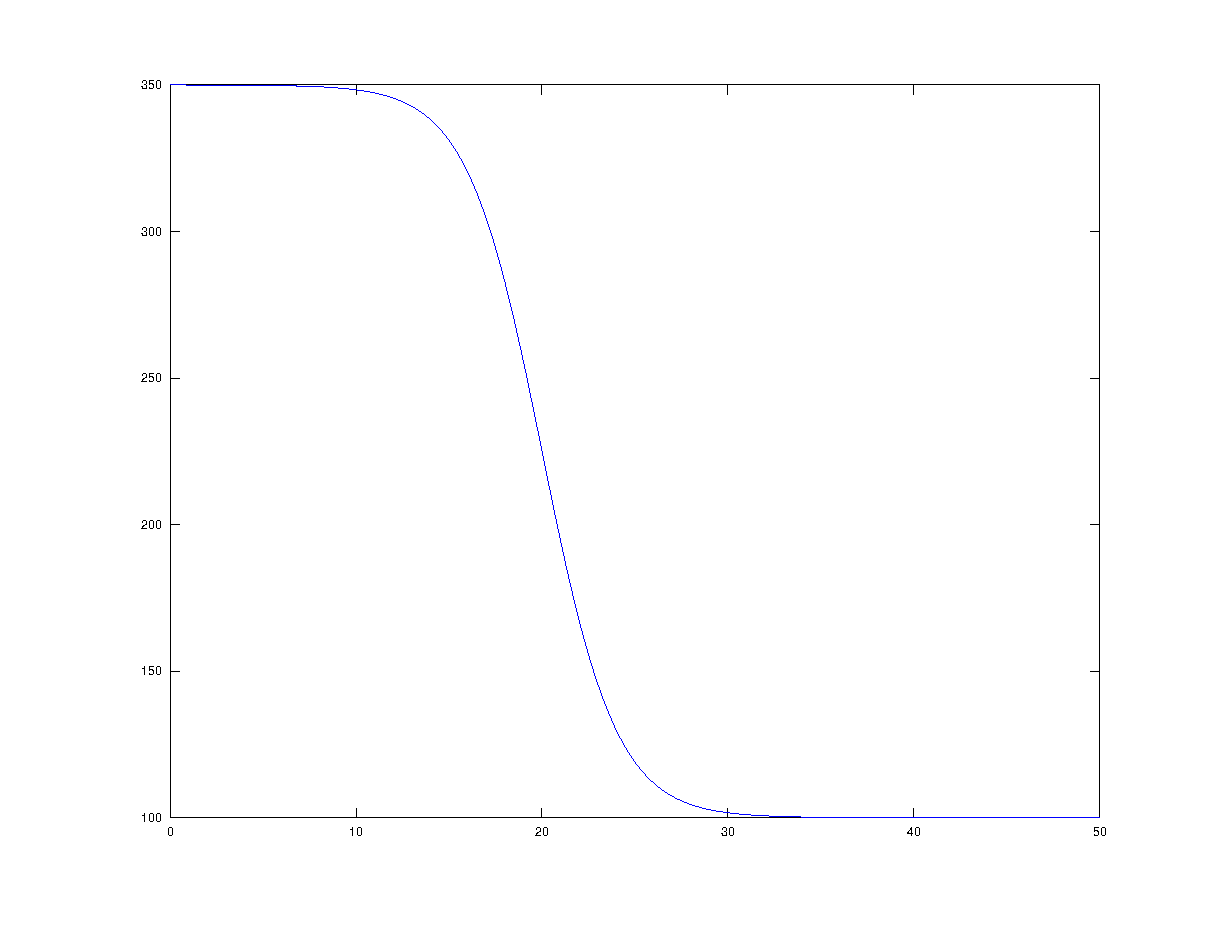
\includegraphics[width=0.95\textwidth]{sigmaPlot.eps}
				%\caption{Demonstration of the value function for changing kappa}
			\end{center}
			\caption{Plot of the altered sigmoid function (eq. \ref{eqAlteredSigmoidFunk}), with \mbox{$c_1$ = 100}, \mbox{$c_2$ = 250}, \mbox{$c_3$ = 10} and \mbox{$c_4$ = 0.5} }
			\label{figAlteredSigmoidFunction}
		\end{figure}
	
		This will give a the largest output value when the error is very small. For increasing errors, the output of the altered sigmoid function will become smaller.
		We can see from plot \ref{figAlteredSigmoidFunction} that the altered sigmoid function \eqref{eqAlteredSigmoidFunk} give a maximal and a minimal period for the recalculation of $\kappa$.
	
		From \eqref{eqAlteredSigmoidFunk} we can see that the altered sigmoid function has the maximum value of $c_1+c_2$.
		In fig. \ref{figAlteredSigmoidFunction} the values $c_1 = 100$ and  $c_2 = 250$, giving the maximum value as 350 time iterations between recalculation of $\kappa$.
		Because of a small degree of truncation error in the small test cases used while testing this implementation, the minimal period between recalculation was set so $c_1=100$ time iterations. 
		This can easily be altered for larger test cases, or other situations where the truncation errors become an issue.
		% TODO Skriv om det under. Blir overflødig..
		%The altered sigmoid function \eqref{eqAlteredSigmoidFunk} is used when the period to the next recalculation of $\kappa$ is planned. 
		%The maximum value, in this context, gives the maximum period before the new recalculation is done. %This happens when the error is wery small (se fig \ref{figAlteredSigmoidFunction}).
		%The minimal and maximal period between recaluclation can be modified by altering the constants $c_1$ and $c_2$.

		%TODO skriv litt om, de neste to avsnitta.
		% TODO SKRIV DETTE, MEN SKRIV OM FØRST :  One other thing that is worth noting is the variables $c_3$ and $c_4$ giving the shape of the curve. $c_4$ gives the lenght of the curve, that is how steep it is.
		


		% TODO TODO TODO TODO TODO TODO TODO TODO TODO TODO TODO TODO TODO TODO TODO TODO TODO TODO TODO TODO TODO TODO TODO TODO TODO TODO TODO TODO TODO TODO TODO TODO TODO 
		% Har rudda i tekst til hit.
		\subsection{------------ Har rydda i tekst, til hit ------------- }

		After some analysis, I desided to use the values used in fig. \ref{figAlteredSigmoidFunction}.
		This gives a function that gives maximum period between recalculation of $\kappa$ when the error is below about 10. 
		It has a relatively steep decent between an error of 10 and 30. The minimum period is set to 100 time steps and the maximum to 350 time iterations.

		The minimum time between recalculation of $\kappa$ will limit the use of resources. %cause the simulation not to use to much resouces.
		The maximum value of this function is limited because the error will have a stocastic nature, and one could e.g. end up with zero error if one get equal positive and negative errors.
		This could potentially give a very large period before the next recalculation of $\kappa$.

		Because of the stocastic element of the trunction error, the planning of the next recalculation of $\kappa$ is also implemented as a FIR--filter with a moving average over the last three values.
		%For this reason, the calculation of the period between recalculation of $\kappa$ is also implemented as a FIR--filter with a moving average over the last three values.
		%
		%When the auron is constructed, $\kappa$ is recalculated before any input synapses is defined. This gives the filter a small initial period.
		When the simulation starts, $\kappa$ is first calculated by the recaluclate function, giving the recalculate function a small initial period based on the level of synaptic input.
		% ELLER MEIR RETT: The first time $\kappa$ is calculated, it is calculated with the recalculate function, giving the filter a small initial period, based on the initial level of input.
		Aurons with a large initial input will therefore get a smaller initial recalculation period that some auron with a smaller initial input. %due to a large initial error.

		\subsection{Implementation of recalculation of $\kappa$}
		The execution of the planned recalculation of $\kappa$ is done in the same way as the execution of the planned action potential for the $\kappa$ auron.
		In the next section I will use some time on evaluating different methods for executing planned events at the planned time.
		The choice of method for this implementation is described in section \ref{ssChoiceOfTimeEstimationForThisImplementation}.
		
		For recalculation of $\kappa$ with the chosen method, we need a separate object whose doTask() function will call the K\_aurons recalculateKappa() function.
		To achieve this, each K\_auron has its own object of the class recalcKappaClass().

		recalcKappaClass::doTask() then will call the associated K\_aurons recalculateKappa() function, in addition to planning the time of the next recalculation according to the considerations in section \ref{ssecRecalcKappa}.
		

% HER EHER HER er eg.

		%Siden kappa bare regnes ut som integralet av den deriverte, vil det være behov for rekalkulering av Kappa, i ny og ne. Dette bør ikkje skje for ofte, heller ikkje for sjeldent.
		%Difor: lage en adaptiv utførelse av dette. Dette sjekker avviket mellom den rekalkulerte verdien og den gjeldende verdien, ved rekalkulering. 
		%
		%Dette avviket sjekkes opp i mot en predefinert ønska verdi, og differansen er med på å bestemme om periode til neste rekalkulering skal auke eller minke (auker/minker som en funksjon av avvik-avviket). 
		%
		%Dette avviket er m.a.o. med på å bestemme tid til neste rekalkulering av Kappa.
		%Auken/minken bør ha en maksverdi.



% KAN ikkje denne takast vekk? XXX XXX XXX
	\subsection{Estimation of firing time}
	% Skriv kvifor eg kaller det "Estimation" og ikkje calculation.
	%TODO dette var en del av section{KANN} tidligere. Fokuset i teksten er det. Skriv om slik at det gjelder generelt, men med spesiellt fokus på KANN.
	For KANN, synaptic transmission can be defined as transmission of change in the postsynaptic node's input level.
	The input of a node, in terms of $\kappa$, is propotional to the synaptic weight and inversly propotional with the presynaptic inter--spike period.

	When the presynaptic node changes its activation level, and its period increases or decreases, the level of synaptic transmission will be altered accordingly. 
	Because of the number of synapses per axon/ dendrite, it is most efficient to perform as many of the calucations as possible in the presynaptic auron.
	For this reason, the most efficient way of calucating the postsynaptic dendrite's activation level is to let the synapse transmit the derived of the signal (change).
	%TODO Har skrevet dette tidligare. (to subsections før). Skriv om, og referer/underbygg denne måten.

	If the transmitted varible is the derived of the signal the postsynaptic dendrite can easily calculate the changed postsynaptic $\kappa_i$, as sen in section \ref{ssecSynInputToANodeKANN}.
	% XXX SAGT FØR: If we define $\kappa_{ij}$ as the contribution on $\kappa_i$ from the synapse between node $j$ and node $i$ , $\kappa_i$ can be calculated as
	%\begin{equation}
	%	\kappa_{i} = \sum_j{\kappa_{ij}}
	%\end{equation}
	
	If every $\kappa_{ij}$ but one, $\kappa_{ix}$, is kept constant, it can be shown that $\Delta \kappa_i$ is equal to $\Delta \kappa_{ix}$.
	Following that $\kappa$ is calculated as a superposition of all the input synapses contribution, these equations can be extended to change of transmission of multiple synapses.
	This gives us the equation for the change of postsynaptic activation level following synaptic transmission at synapse from node $x$ to node $i$.

	\begin{equation}
		\kappa_{ij, new} = \kappa_{ij, old} + \Delta \kappa_{ij}
	\end{equation}

	Instead of calculating all of this at every synapse, or for every synapse at the postsynaptic dendrite, it is better to calculate as much as possible presynapticlly.
	This gives one calulation every time a node fires an action potential, instead of one for every output synapse.

	%XXX XXX XXX Trur eg skrive  resten i subsubsection: implementation:KANN -> pEstimatedTaskTime -> execution of elements
	
	% TODO SKRIV litt om dette her, og lag eit frampeik til etter pEstimatedTaskTime, der eg skal skrive meir om dette.
	%Transmission of the derived solves many problems concerning efficiency, but it also introduces integral error for the postsynaptic $\kappa_i$
	%This problem can be solved, and we will come out JAJAJ. Skriv anna gang-- TODO


	%Etterkvart: skriv om integral-errors og fiksing av dette ved å bruke pEstimatedTaskTime (regelmessig fiksing, som er adaptiv med basis i feilen på postsyn signal (høg feil=>oftere regelmessighet på resumming av kappa)).


	When the firing time is estimated, it is fundamental that we have a mechanism for executing these elements at the right time. 
	In the section \ref{secPlannedEvents} two different solutions has been proposed for this. 
	The section is concluded by presenting a discussion behind the choice for this implementation.
	%XXX BLÆ! skriv om linja over!
	%In section \ref{ssChoiceOfTimeEstimationForThisImplementation} the choice for this implementation will be presented, and different pros and cons with each method will be discussed.



%	\subsection{When do $\kappa$ propagate?} %TODO TODO Dette er analyse => Discursion! XXX XXX XXX XXX XXX XXX XXX XXX XXX XXX XXX XXX XXX XXX XXX XXX XXX XXX XXX XXX XXX XXX XXX XXX XXX XXX XXX XXX XXX XXX XXX XXX XXX 
%	In the start of this project, $\kappa$ANN were implemented as a varian of a network with spiking nodes.
%	Here the information is transmitted by the synapses following an action potential. 
%	Because the SANN model was the basis of this implementation, the information were originally transmitted at the time of the node spiking.
% %XXX XXX XXX XXX XXX XXX XXX XXX XXX XXX XXX XXX XXX XXX XXX XXX XXX XXX XXX XXX XXX XXX XXX XXX XXX XXX XXX XXX XXX XXX XXX XXX XXX XXX XXX XXX XXX XXX XXX XXX XXX XXX XXX XXX 	
% %FORTSETT HER
%	ARGUMENTER for at den propagerer heile tida.
%Stavdal meiner at det er tull å propagere heile tida (kvar gang K oppdateres i presyn). 
%Eg har laga plot for å sei imot dette: når kappa venter med å propagere til første fyring får man eit tidsdelay for depol til KN tilsvarende tida det tar til første fyring. (dette er veldig tydlig ved sprang i presyn K).
%
%Når Kappa propagerer kvar gang presyn endres, fjærnes dette problemet. Propagerer som det er gjordt før, med at axon legges til i pWorkTaskQue. Alle postsyn. noder får dermed input tidligst neste iterasjon.
%
%Dette har med synapstisk transmissjon å gjøre, og eg må gjøre dette ferdig før eg skrive meir om dette..
%
%NEI faen! no er feilen der igjen. Sjekka kode, og fann at den propagerete, men bare om K>T, så det over er TULL.
%

% TODO TODO TODO TODO TODO TODO TODO TODO TODO TODO TODO TODO TODO TODO TODO TODO TODO TODO TODO TODO TODO TODO TODO TODO TODO TODO TODO TODO TODO TODO TODO TODO TODO TODO TODO TODO TODO TODO TODO TODO TODO TODO TODO TODO 
% Lag plott av KN for nettverk der sensorneuronet venter til fyring, og eit SN depol-plott. For sammenligning (chap. comparison and results).
% TODO TODO TODO TODO TODO TODO TODO TODO TODO TODO TODO TODO TODO TODO TODO TODO TODO TODO TODO TODO TODO TODO TODO TODO TODO TODO TODO TODO TODO TODO TODO TODO TODO TODO TODO TODO TODO TODO TODO TODO TODO TODO TODO TODO 

























% //{ \section{Planned Events}
%	\label{secPlannedEvents}
%	\subsection{pEstimatedTaskTime}
%	$\kappa$ANN is based on calculating the firing time, given the present level of input. 
%	Because the input level of an ANN node varies constantly, the calculated firing time is but an estimation of the nodes firing time. 
%	The estimation of the nodes firing time changes as the input level does.
%	%The estimated firing time for a node changes as the input level does.
%	
%	The std::list pEstimatedTaskTime is basically an array of dynamic size consisting of std::list--elements,
%	where the outer list is an array of future time iterations and the inner lists are arrays of tasks estimated for the respective future time iterations.
%	%The inner list is an array of tasks, the outer list is an array of future time iterations. 
%	%This can be used for planning the time of execution for different tasks.
%	%that keeps overview of when the tasks in the inner tasklist is to be executed.
%
%	The outer list could be said to be the time iteration (relative to the present time iteration) when the tasks in the conlaining list are to be performed. 
%	When every task in the inner task list is completed, % ELLER "moved to the pWorkTaskQue" 
%		the task list is removed from the outer list. 
%	In this way it is possible to keep the relative time--task list updated.
%
%	The tasks located in the inner list of the first element of the outer list are the tasks that are to be executed the next time iteration.
%%	Tasks that are to be performed the next time iteration is inserted in the first element (inner list) of the outer list.
%%	In time\_class::doTask(), the first element of the outer list (the first inner list) is evaluated, and all the taskt are executed. 
%	time\_class::doTask() is responsible for tasks being executed at the planned time. 
%	Before time\_class::doTask() iterates time (and moves its pointer from the first element to the last element of pWorkTaskQue), all tasks that are planned for next time iteration is moved from pEstimatedTaskTime to pWorkTaskQue.
%	The tasks are appended at the back of pWorkTaskQue before the time\_class object pointer is moved to the end of pWorkTaskQue. 
%	This will cause the planned tasks to be performed the next time iteration.
%
%%	Before the discrete time is iterated, the first element is removed from the outer pEstimatedTaskTime--list.
%%	In this way it is possible to keep an overview of the immediate future with pEstimatedTaskTime.
%
%	If a new element (a new task) is to be inserted somewhere outside the present scope of the pEstimatedTaskTime, the element (std::list) needs to be constructed.
%	Because of the mechanisms of pEstimatedTaskTime, not only the element needs to be produced but also all the estimated time iterations between the length of pEstimatedTaskTime and the estimated time of the respective task.
%
%%dette står lenger nede, under "insertion of elements"
%%\begin{lstlisting}
%%int nDiff = uRelativeTime - pEstimatedTaskTime.size();
%%if( nDiff >= 0 ) //Mangler ledd. Legg til rett antall.
%%{
%%  for(int i=0; i <= nDiff; i++){
%%  pEstimatedTaskTime.push_back( new std::list<timeInterface*> );
%%  }
%%}
%%\end{lstlisting}
%	
%	\subsubsection{Insertion of elements}
%	The std::list container is implemented as a doubly linked list\cite{Stroustrup2000KAP16}.
%	To find element nr. $n$ we can iterate throught the list $n$ times from the beginning.
%% 	To find element nr. $n$ we can either iterated throught the list ($n$ times) from the beginning, or $S-n$ iterations from the end.
%%	An alternative approach if we are concerned with efficiancy, is to iterate from the end that is closest to the element (the beginning or the end of the list).
%	In doubly linked lists, we can also iterate thourgh the list from the end.
%	If we always iterate from the end that is closest to the target element, the number of iterations required will be halved (if the target position is completely random within a fixed--size list).
%
%	If, for example, we have a list that is 10 elements long and want to access element nr. 9, the most efficient way of doing this in a doubly linked list is to start at the end.
%	To generalize this, we can say that if the element that needs to be accessed is later than $\frac{[\text{size of list}]}{2}$ the ``search'' will start at the end.
%
%\begin{lstlisting}
%if( uRelativeTime_arg < (pEstimatedTaskTime.size())/2 ){
%  // Seach from the last element.
%}else{
%  // Seach from the first element.
%}
%\end{lstlisting}
%
%	%If, however, the estimated task time is outside the scope of pEstimatedTaskTime, new elements will have to be inserted.
%	Insertion of tasks outside the immediate length of pEstimatedTaskTime requires some attention.
%	When an event is planned for some time iteration outside the scope of pEstimatedTaskTime, the scope of pEstimatedTaskTime will have to be increased.
%	Because the pEstimatedTaskTime works as a FIFO--que, where the first element % (containing a list of all the planned tasks for the future time iteration)  (se section \ref{ssecEvaluationOfpEstimatedTaskTimeELEMENTS})
%		is popped in time\_class::doTask(), it is important to insert every element between the present scope of pEstimatedTaskTime and the new planned task time.
%	This is done by
%\begin{lstlisting}
%int nDiff = uTimeToTask-pEstimatedTaskTime.size();
%if( nDiff >= 0){
%  for(int i=0; i<=nDiff; i++)
%    pEstimatedTaskTime.push_back( new std::list<timeInterface*> );
%}
%\end{lstlisting}
%%This algorithm enshures that pEstimatedTaskTime is correct in terms of time planning.
%The expression in the for loop is the reason for having the outer elements of pEstimatedTaskTime defined as std::list$<$timeInterface*$>$ pointers.
%In the above algorithm, new std::lists are created in the free store. This creates elements for pEstimatedTaskTime that will exist after the return from the function where the elements are constructed.
%%When the free store is used, it is important to deallocate the memory after the element is used. %skriv bedre, denne setininga
%To avoid memory exhaustion, it is important to deallocate the memory allocated in the free store when the variable no longer will be used. This is done when the inner lists are evaluated in \emph{time\_class::doTask()}.
%For more about the execution of pEstimatedTaskTime tasks, se section \ref{ssecEvaluationOfpEstimatedTaskTimeELEMENTS}.
%%TODO Skrim om deallocating memory i ssecEvaluationOfpEstimatedTaskTimeELEMENTS   asd123
%
%
%	%TODO Koden for denne insertion--funksjonen skal være med i appendix!
%	% 			- og skal refereres til fra [her]
%
%
%
%%
%% 	Skriv om at funk får inn relativ tidsflytt som argument. For å finne relativ tidsflytt trenger eg å lagre gammelTidsPkt i timeInterface-objekt.
%% 	Skriv om iterator opplegg. Iterator-returnerende funksjon som søker seg fram til rett ytre-liste (fremtidig tidsiterasjon..)
%
%	\subsubsection{Moving tasks in pEstimatedTaskTime}
%	When the planned task time for a timeInterface object is changed, the pointer to the object have to be moved in the pEstimatedTaskTime list.
%	
%	%In the standard library containers, pointers to elements are called iterators. An iterator 
%
%% TODO TODO TODO TODO TODO TODO TODO TODO TODO TODO TODO TODO TODO TODO TODO TODO
%% TODO TODO TODO TODO TODO TODO TODO TODO TODO TODO TODO TODO TODO TODO TODO TOD
%% TODO TODO TODO TODO TODO TODO TODO TODO TODO TODO TODO TODO TODO TODO TODO TO
%% TODO TODO TODO TODO TODO TODO TODO TODO TODO TODO TODO TODO TODO TODO TODO T
%	%TODO lagre heller iteratoren i timeInterface objektet. Tar langt mindre tid. Trur det at iteratoren blir invalidated bare gjelder for vector..
%	XXX KORLEIS skal eg gjøre dette? No lagrer eg ulTid i objektet. Kanskje eg heller skal lagre list<list*>::iterator ? Funker dette bedre?
%	\emph{Det er bare for vector at iteratoren blir ivalidated når størrelsen på container endre!}
%
%	%Uavhengig av korleis eg finner element, kan eg skrive om flytting av element:
%	When the estimated task time is altered, one can assume that the new position will be located not far from the old position, compared to the size of the whole pEstimatedTaskTime list.
%	In this case, the most efficient way of finding the new position is to iterate $x$ positions from the old estimated time iteration in pEstimatedTaskTime, instead of finding the position from one of the ends of pEstimatedTaskTime.
%	The relative moval of the task can be desided by taking the difference between the new estimate and the old estimate of the task time, $x$, and move the object pointer $x$ iterations along pEstimatedTaskTime. 
%	$x$ may be positive or regative.
%	
%%	\subsubsection{Flytting av element}
%%	Implementer først, så skriv om flytting av element som resultat av ny $\kappa$.
%%	Element vil ikkje flyttes langt, så beste vil være å flytte elementet fra [no-posisjon].
%%	Dette kan lett gjøres i ei `doubly linked list'.
%%
%%	(planen no er å flytte den ved å ta inn no-iterator-plass (som er lagra i K\_auron) og kor langt den skal flyttes. 
%%	Dette gjøres best ved å overlagre funksjonen for når den får argument (iter, timeInterface, tidsFlytt). 
%%	Bør returnere iterator, for at auronet skal ha muligheten til å lagre også ny iterator i pEstimatedTaskTime).
%
%
%
%
%	\subsubsection{Evalutation of pEstimatedTaskTime elements}
%	%\subsubsection{execution of element tasks}
%	\label{ssecEvaluationOfpEstimatedTaskTimeELEMENTS}
%
%	%pEstimatedTaskTime: where all planned tasks for future time iteration lies,
%	%pWorkTaskQue: where the tasks for the immediate future lies.
%	When the time iteration for the planned events in pEstimatedTaskTime arrives, the tasks in the pEstimatedTaskTime element need execution.
%
%	This can be done by executing the tasks in a separate function, e.g. time\_class::doTask(), that is called at an ideal time for evaluating pEstimatedTaskTime elements.
%	%time\_class::doTask() is ideal for executing the tasks. 
%	To be consistent about the execution of tasks, it is better to move the tasks planned for the next time iteration from the next element in pEstimatedTaskTime to the pWorkTaskQue list.
%	pWorkTaskQue is the list used to plan the immediate future for the ANN, initially developed for the SANN model that focus more on the immediate state of the system.
%
%	When this is done in time\_class::doTask() before time is iterated and the time\_class time separation object is moved to the end of pWorkTaskQue, the tasks from pEstimatedTaskTime will be executed the next time iteration.
%	%When the estimated time for the elements task is at the next time iteration, time\_class::doTask() will insert a pointer to the element into pWorkTaskQue.
%	%This will will call the node elements \emph{doTask()} function the next time iteration. 
%
%%	The elements of pEstimatedTaskTime is created in the free store, and needs to be deallocated to avoid memory exhaustion. 
%	When a pointer to an element is removed from pEstimatedTaskTime, the elements destructor is not called. 
%	%When an element is removed from pEstimatedTaskTime, the value of the dereferenced elements destructor is not called because the element is a pointer. 
%	It is therefore important to deallocate the memory used for the object in the free store to avoid memory exhaustion.
%	%When the element us used and no longer needs to be stored, 
%	At the end of time\_class::doTask() this is done explicitly:
%\begin{lstlisting}
%delete pEstimatedTaskTime.front();
%pEstimatedTaskTime.pop_front();
%\end{lstlisting}
%	The \emph{delete} operator frees the memory allocated to the task list planned for the next time iteration (the dereferenced pointer)
%	and the \emph{pop\_front{}} operator removes the now empty pointer in the first element of \emph{pEstimatedTaskTime}.
%
%
%	
%
%% TODO Skrive eksempel med "the action potential cascade? :
%	%I will in the remainder of this section focus on the action potential cascade. 
%	%When the firing time of the auron is estimated, a pointer to the auron node element is inserted into pEstimatedTaskTime. 
%	%When the time comes for the auron to fire an action potential, the auron pointer is interted into pWorkTaskQue, and the \emph{K\_auron::doTask()} will be executed at the estimated time iteration, inducing the action potential cascade.
%
%	%For K\_aurons, the \emph{doTask()} will first calculate the aurons inverse period (``instantaneous frequency''). 
%	%The result is variable \emph{K\_auron::uLastCalculatedPeriod} is made to save this value for later use.
%	
%	%The new period is calculated, using equation \eqref{eqPeriodeligningForKonstIntraPeriodKAPPA}, giving the level of transmission at the nodes output synapses.
%	
%	%skriv litt om at denne ligninga er basert på konst. interspike kappa. Dette har vi ikkje her. Kvifor er det viktig alikevel. 
%	% 	- delay i ANN. Vente på første spike kan være uoptimalt, men det vil være proposjonalt med aktiviteten, som kan være bra. osv. Drøft (seinare, nevne det her..)
%	% 	- arbeidsbelastning.
%	
%
%	%\subsection{Checking a member variable of timeInterface--derived elements}
%	%TODO Finn bedre tittel for dette!
%	\subsection{Checking estimated task time directly from time\_class::doTask()}
%	A more direct approach is to check the elements estimated firing time directly from time\_class::doTask(). 
%	Every class derived from timeInterface contains a variable called ulEstimatedTaskTime where the elements estimated task time is written every time this is updated.
%	If we check ulEstimatedTaskTime every time iteration, and number is the same as the next time iteration's index (ulTime), time\_class::doTask() is responsible to insert its pointer into pWorkTaskQue.
%	This will cause the element to do its task on the planned time iteration.
%	%If lEstimatedTaskTime is the same as the next time iterations ulTime, we can insert a pointer to the element into pWorkTaskQue, causing it to do its task next time iteration.
%
%	When $\kappa$ is updated, and K\_auron::doCalculation() updates the aurons estimated firing time, it also updates the K\_auron::lEstimatedTaskTime.
%	If $\kappa$ is less than the firing threshold, the K\_aurons lEstimatedTaskTime is set to 0. 
%
%	\subsubsection{Execution of elements}
%	time\_class::doTask() runs through the list K\_auron::allKappaAurons to see if any elements have an estimated firing time the next iteration.
%	When it finds an element scheduled for the next iteration, the pointer to the element is imnserted into pWorkTaskQue.
%
%
%	\subsection{The Choice for this Implementation}
%	\ref{ssChoiceOfTimeEstimationForThisImplementation}
%	% XXX TODO BEGRUNN GODT KVIFOR EG HAR SKREVET SÅ MYKJE OM pEstimatedTaskTime! Det holder ikkje at eg har gjordt det.
%	% 	Skriv at det er godt mulig dette er den mest effektive algoritmen når antall noder auker kraftig!
%	% 	Skriv at i såfall må en maks-lengde på lista lages.
%	The two methods for execution of tasks at the planned time both have flaws and cons.
%	
%	pEstimatedTaskTime krever at alle flyttinger av element er riktig. Dersom det er mykje endring av kappa er dette dårlig for denne metoden (krever mykje flytting av element i pEstimatedTaskTime).
%	Denne lista er derimot heilt uavhengig av antall auron vi simulerer. For store ANN vil nok denne pEstimatedTaskTime-varianten være best.
%
%	Dersom vi har endring av kappa heile tida, kan metode 2 (den direkte metoden) være best.
%	Da koster det ikkje noke å endre fyringsestimatet, men man har en konstant 'cost' ved iterasjon av tid. (BEMERK AT DENNE ER const SEINARE)
%	Denne 'cost' er avhengig av antall K\_auron (da den må iterere gjennom alle element [med K>T?]). Denne 'cost' er constant for eit gitt antall auron.
%
%	Det er to grunner til at eg har valt den siste metoden: 1) mine ANN vil være små med mykje endring av kappa. Dette gjør at det er heilt forsvarlig å velge metode nr. 1.
%	Den andre grunnen til at eg velger metode nr.1 er at denne har konstant timedelay, noko som er bra..
%
%	jeje... Osv.
%
%	For this implementation, both methods were implemented and tested. 
%
%
%
%
%
%
%
%
%
%
%
%
%
%
%
%%	\subsection{Anna fra tidligare:}
%%	-- kanskje skrive om vanskene med log() ? Returnerer samme som argumentet, difor må vi typekonvertere til (float) eller (double) før man tar log() av det. Dette skapte hodebry, siden eg bare fekk resultatet 0.
%% TODO Skrive om dette i konslusjon. Dette er (veldig små) eksempel på vanskene med KANN. Kan nevnes såvidt (som i ei halv setning, f.eks.)
%% 		Ganga med FAKTOR, og fekk 0. Når eg typekonverterte argumenta til log() om til float gjekk fekk eg bra output..
%
%%	Skriv også om at istedenfor å skrive $t_{estimert} = - \frac{1}{\alpha} \ln(\frac{\kappa-\tau}{\kappa-v_0})$ kan eg skrive $t_{estimert} = \frac{1}{\alpha} \ln(\frac{\kappa-v_0}{\kappa-\tau})$
%%	(ferre operasjoner, meir effektivt!).
%
%%	\subsection{simulering vha. ligning \eqref{eqVerdiligninga} fra section \ref{secMatematiskModelleringAvBioNeuron}}
%%	\subsection{Osv.}
%
%
%
%
%
%
%
%
%
%%antagligvis her, men veit ikkje heilt. Iterators. Brukes mykje, så bør forklares (spess for en C patriot)
%%\subsection{Skriv om iterators, en plass}
%%Dette er veldig viktig for produktet, så bør skrives om.
%%
%%Iterators er en høgare form for peiker. 
%%I standard library er mange basisfunksjoner implementert, og små operatorer (som lenka liste iterering) er lett å implementere.
%%Mange små funksjoner som er lett å implementere får alle en liten sannsynlighet for feil. Når det er mange av desse får man mange potensielle feil som er vanskelig å finne.
%%
%%I standard library er blandt anna en del "containers", som list. Dette er ei ``doubly linked list''.
%%Man har også såkalla ``iterators'', som er en peiker til element i slike containers.
%%Desse har blandt anna implementert iterator operatoren \emph{++}. Denne er garantert feilfri, og bør brukes fremfor å imlementere slikt selv (seier stroustrup)[referere!].
%%
%%Skriv at i tillegg til at man kan gå ut  fra at de er feilfri, så er de også godt optimalisert, og vil ofte gi en meir effektiv implementsjon.
%%
%%Iteratoren har veldig masse til felles med en peiker, bare med lettere, feilfri, meir optimalisert utførelse.
%
%
%%\subsubsection{Ikkje mulig å lagre iteratoren}
%%ELLER ER DET MULIG? (Kan være det under bare gjelder for vector!)
%%
%%Iteratore blir ugyldige, og gir udefinert oppførsel dersom lista blir rezised i mellom iteratoren blir laget og brukt. 
%%Initiellt var tanken at K\_auron (og kanskje andre timeInterface som bruker pEstimatedTaskTime) skulle også inneholde en iterator (peiker) til rett element i lista.
%%Siden iteratore blir ugyldig når listas lengde endres %stroustrup s. 550, nede. Understreka.
%%	så går ikkje dette.
%%
%%Dette er grunnen til at kvar gang eit element skal flyttes, må det søkes opp på nytt (forrige plass kan inneholde eit nytt element, eller være forbi slutten av lista..)
%%
%%Siden vi ikkje bør anta kor den er, bør lista itereres gjennom på nytt. 
%%En antagelse som er trygg er at elementet ikkje har flyttet seg veldig langt, når estimatet oppdateres.
%%Dette gjør at det antagelig ligger i samme halvdel av lista, og det kan være lurt å begynne søket fra den siden som er nærmast ny plassering. %type før eller etter size() / 2 , før => start søk fra starten ...
%%
%%For å effektivisere, lages to funksjoner: en som legger til element, og en som flytter det. 
%%Ved fyring av K\_auron fjærnes elementet, men skal også legges til på tidspkt. [no]+[estimert periode].
%%Løsninga mi blir: i funksjonen som fjærner elementet, vil også nytt element legges til om element->periode. Dette er en rein insertion.
%%
%%For flytting av element må lista itereres gjennom, og kvar iterasjon må lista--elementet gjennomsøkes etter gjeldende element. 
%%Dette er meir tidkrevende, og er grunnen til at eg skiller mellom de to operasjonene: insertion og moving of an element.
%%
%%Les stroustrup s. 550 for meir, når dette skal skrives om!
%
%
%
%
%
%
% //}
